\chapter{CPUの仮想化}
\label{tacosVirtualCPU}
実例としてTacOS\footnote{TacOSの詳細は
  \url{https://github.com/tctsigemura/TacOS}
  を参照のこと.}の例を紹介する.
TacOSはマルチプロセスのオペレーティングシステムである.
以下ではCPUの時分割多重に必要なプロセス切換え機構を紹介する.

%==============================================================================
\section{PCB}
PCBはプロセス切換え機構にとっても最も重要なデータ構造である.
TacOSのPCBはリスト\ref{tacosPCB}に示す
\|PCB|構造体として定義されている\footnote{
  \url{https://github.com/tctsigemura/TacOS/blob/master/os/kernel/process.hmm}
  の一部である.}.
\|PCB|構造体の内容を順に説明する.

\lstinputlisting[firstline=68,lastline=96,numbers=left,label=tacosPCB,
  float=btp,caption=TacOSのPCB宣言ソースプログラム]{TacOS/kernel/process.hmm}

\begin{itemize}
\item 仮想CPU(\|sp|) \\
  TacOSはプロセスのコンテキストのほとんどをカーネルスタック上に保存する.
  そして,保存位置を表すスタックポインタ(SP)だけをPCBに保存する.
  カーネルスタックはプロセス毎に準備されている.
  PCBに保存されるのは仮想CPUの一部(SP)だけである.
\item プロセス番号(\|pid|)
\item 状態(\|stat|) \\
  TacOSのプロセスの状態は以下の三つである.
  \begin{enumerate}
  \item \|P_RUN| \\
    RunningとReadyの二つを兼用している.
    プロセスは実行可能プロセスの待ち行列(実行可能列)に挿入される際に
    \|P_RUN|状態になる.
    実行中も\|P_RUN|状態のまま変更しない.
  \item \|P_WAIT| \\
    Waiting状態のことである.
  \item \|P_ZOMBIE| \\
    プロセスが終了したが,終了ステータスを親プロセスに渡していない状態である.
    終了処理の途中状態と考えるとよい.
  \end{enumerate}
\item 優先度(\|nice|,\|enice|) \\
  ゼロが最も高い優先度を表す.
  優先度には,
  本来の優先度(\|nice|)と,
  実質の優先度(\|enice|)の二つがある.
  現在の実装ではこの二つは同じ値を持つ.
  将来,動的に変化する優先度を採用する場合に,
  \|enice|の値が変化するようにする.
\item プロセステーブルのインデクス(\|idx|) \\
  このPCBが登録されているプロセステーブル内の位置である.
  プロセスが消滅する際にプロセステーブルからPCBを削除するために使用する.
\item イベント用カウンタとセマフォ(\|evtCnt|,\|evtSem|) \\
  セマフォはプロセス間の同期に使用する基本的な機構である\footnote{
    詳しくは後の章で解説する.}.
  タイマー待ち,子プロセスの終了待ち等で,
  このセマフォを使用してプロセスを待ち状態にする.
  カウンタはタイマーの待ち時間を計るため等に使用される.
\item プロセスのアドレス空間(\|memBase|,\|memLen|) \\
  TacOSには仮想記憶のような高度な機構は無い.
  各プロセスは,
  物理メモリの領域をオペレーティングシステムによって割付けられる.
  \|memBase|は
  オペレーティングシステムがプロセスに割当てたメモリ領域の開始アドレス,
  \|memLen|はメモリ領域のバイト数である.
\item プロセスの親子関係の情報(\|parent|,\|exitStat|) \\
  TacOSのプロセスは親プロセスだけ記憶している.
  \|parent|は親プロセスのPCBを指すポインタである.
  \|exitStat|は\|P_ZOMBIE|状態になった時,
  親に渡すべき終了ステータスを保存する領域である.
\item オープン中のファイル一覧(\|fds|) \\
  プロセスがオープンしたファイルのファイルディスクリプタ(番号)の
  一覧を記憶する配列である.
  TacOSではシステム全体で一意なファイルディスクリプタ(番号)が
  用いられる\footnote{
    UNIXのファイルディスクリプタ(番号)はプロセス毎に0番から割振られる.}.
  \|close()|システムコールは,
  クローズするファイルディスクリプタが正当なものか調べるために,
  この配列を使用する.
  \|exit()|システムコールは,
  プロセスを終了する前にプロセスの全オープンファイルをクローズするために,
  この配列を使用する.
\item PCBリストの管理(\|prev|,\|next|) \\
  TacOSはプロセスのリストをPCBのリストとして表現する.
  TacOSのPCBリストは番兵付きの重連結環状リストである
  (\figref{tacosReadyQueue}参照).
  \|prev|,\|next|はリスト上で前後のプロセスのPCBを指すポインタである.
\item スタックオーバーフローの検知(\|magic|) \\
  TacOSはPCBの直後にプロセスのカーネルスタックを配置する.
  万一,カーネルスタックがオーバーフローするとPCBが後ろから破壊される.
  \|magic|はそれを検知するために使用される.
  TacOSはPCBを初期化する際に\|magic|に\|0xabcd|を格納する.
  カーネルスタックがオーバーフローすると,まず,\|magic|領域が破壊される.
  \|magic|の値が変化していないかチェックすることで,
  カーネルスタックのオーバーフローを検知することができる.
\end{itemize}

%==============================================================================
\section{実行可能列}
TacOSの実行可能列は,
\figref{tacosReadyQueue}に示すようなPCBの番兵付き重連結環状リスト
(双方向循環リスト)ある.

\begin{myfig}{btp}{TacOSの実行可能列}{tacosReadyQueue}
  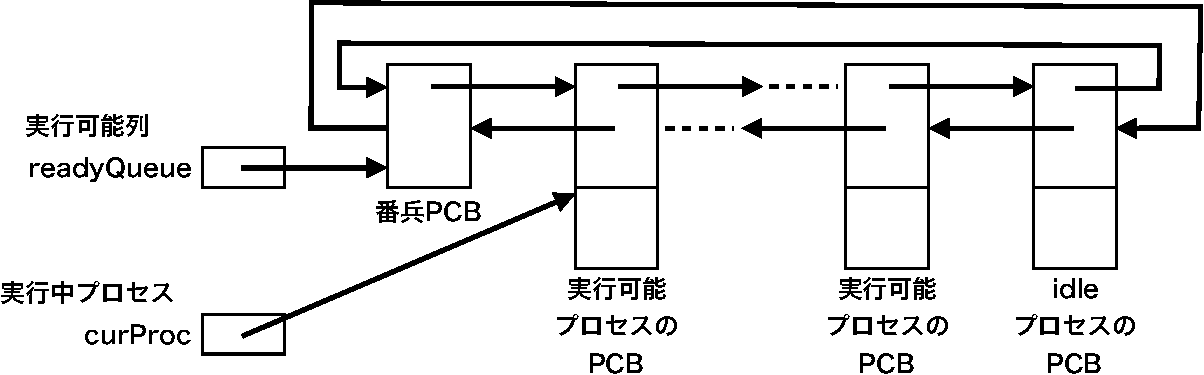
\includegraphics[scale=0.6]{Fig/tacosReadyQueue-crop.pdf}
\end{myfig}

番兵の次のプロセスが最も優先度が高い実行可能なプロセスである.
プロセスをディスパッチする際は,番兵の次のプロセスを選択する.
選択されたプロセスを\|curProc|が指すように変更してからディスパッチする.
TacOSは,PCBを実行可能列に置いたままプロセスを実行する.

プロセスがブロックする際は,
\|curProc|を実行可能列から削除しイベントの待ち行列に移動する.
次回のディスパッチでは,
再度,実行可能列の優先度が最も高いプロセスを選択し,
\|curProc|が指すように変更する.

%==============================================================================
\section{メモリ配置}
\figref{tacosMemMap}にTacOS実行時のメモリマップを示す.
図は二つのプロセスが実行中の例である.
まず「物理メモリ空間」の配置について,
次に「PCBとカーネルスタック」について説明する.

\begin{myfig}{btp}{TacOSのメモリ配置}{tacosMemMap}
  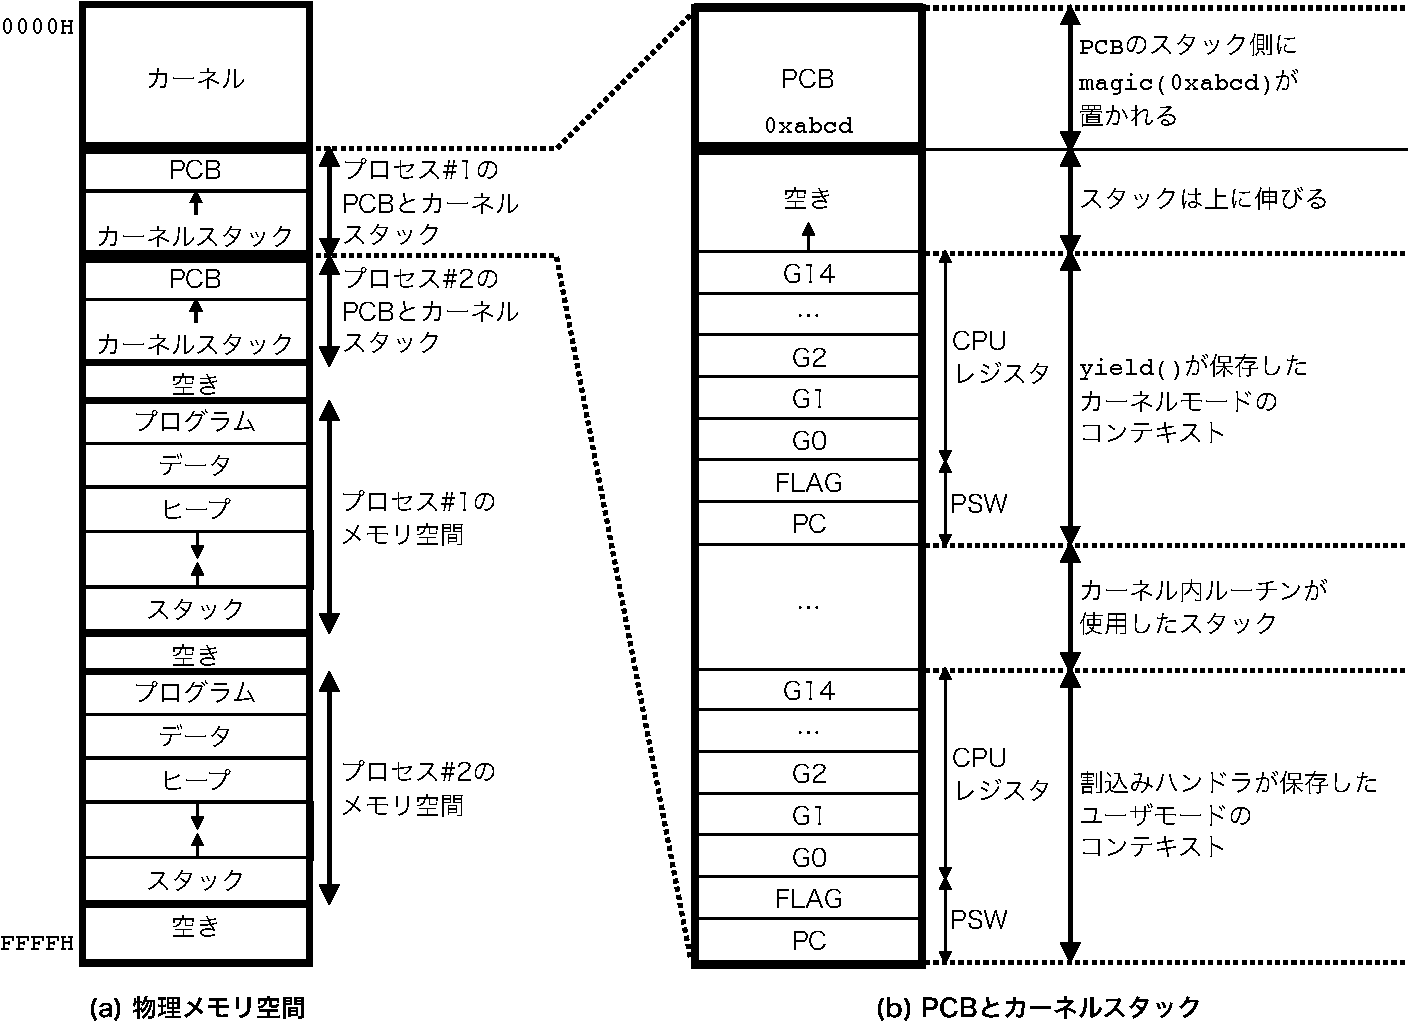
\includegraphics[scale=0.6]{Fig/tacosMemMap-crop.pdf}
\end{myfig}

\begin{enumerate}
\item[(a)] 物理メモリ空間
  \begin{itemize}
  \item カーネル \\
    カーネルのプログラムとデータ(変数)がこの領域に配置される.
  \item プロセス#1のPCBとカーネルスタック \\
    プロセス1のPCBとカーネルスタックが隣接して配置される.
    詳細は\figref{tacosMemMap}(b)に示してある.
  \item プロセス#2のPCBとカーネルスタック \\
    プロセス毎にPCBとカーネルスタックが準備される.
  \item プロセス#1のメモリ空間 \\
    プロセス1のプログラム,データ,ヒープ,スタック領域が配置される.
    ユーザモードのプロセスは,
    この範囲以外のメモリをアクセスできないように保護すべきである.
    しかし,TaCはメモリ保護機構を持っていない.
  \item プロセス#2のメモリ空間 \\
    プロセス毎にメモリ空間が準備される.
  \end{itemize}
\item[(b)] PCBとカーネルスタック \\
  PCBとカーネルスタックはプロセスの生成時に隣接して領域が確保される.
  ユーザプログラム実行中はスタックの内容が空になる
  (スタックポインタがスタック領域の最大アドレスを指す.).
  割込みが発生すると自動的にPSWがカーネルスタックに保存され,
  実行モードがカーネルモードに切換わる.
  次に割込みハンドラに制御が移りCPUレジスタをスタックに保存した後,
  カーネル内ルーチンの実行が始まる.
  カーネル内ルーチンは,PCBに向かって伸びるカーネルスタックを使用する.
  そこで,PCBの最もスタック寄りにマジックナンバー(\|0xabcd|)を配置し,
  スタックが伸びすぎPCBを破壊したことを検知するために使用する.
\end{enumerate}

%==============================================================================
\section{割込み処理}
\label{tacosInterrupt}
TaCはベクタ方式の割込み機構を持っており,
割込み原因毎に割込みハンドラを登録することが可能である.
割込みが発生するとTaCのCPUは次の処理を自動的に行う.

\begin{enumerate}
\item カーネルスタックにPSWを保存する.
\item CPUをカーネルモードかつ割込み禁止に設定する.
\item 対応する割込みベクタに登録されているハンドラにジャンプする.
\end{enumerate}

以下では,タイマー割込みを例に割込みハンドラの振舞いと,
割込み発生時のカーネルスタックの状態を説明する.
リスト\ref{tacosTmr}\footnote{
  \url{https://github.com/tctsigemura/TacOS/blob/master/os/kernel/kernel.cmm}
  の一部である.
}にTacOSのタイマー管理プログラム部分を示す.

\lstinputlisting[firstline=463,lastline=491,numbers=left,label=tacosTmr,
  float=btp,caption=TacOSのタイマー管理プログラム]{TacOS/kernel/kernel.cmm}

\begin{itemize}
\item \emph{割込みハンドラの初期化} \\
  \|tmrInit()|関数はOS起動時に実行され,
  割込みハンドラ(\|tmrIntr()|)関数を
  \|0xffe0|番地から始まる割込みベクタに登録し,
  タイマーのハードウェアを起動する.
\item \emph{割込みハンドラ} \\
  \|interrupt|型の\|tmrIntr()|関数が割込みハンドラである.
  \|interrupt|型の関数は自動的にコンテキストをスタックに保存する.
  自動的に保存されたコンテキストは\figref{tacosMemMap}(b)に示したものである.
  多くの場合ユーザモードで実行中に割込みが発生するので,
  \figref{tacosMemMap}では分かりやすさのためにユーザモードのコンテキストと
  している.

  \|tmrIntr()|関数はプロセステーブルの全てのプロセスについて(8行),
  タイマーの残り時間が0以下になるものを起こす(14行).
  タイマー待ちのプロセスはPCBの\|evtSem|セマフォを用いてブロックしているので,
  \|iSemV()|関数\footnote{
    リスト\ref{tacosSemV}参照
  }を用いてプロセスを起こす.

  最後に,プロセス切換えの可能性があるなら\|yield()|関数\footnote{
    \ref{tacosProcSwitch}で詳しく説明する.
  }を呼び出し,
  プロセスを切り換えるチャンスを作る.
  プロセスが切り換わった場合は,20行を実行中の状態でプロセスがブロックする.
  21行で\|interrupt|関数が終了し,コンテキストが復元され,
  割込まれたプログラムが再開される.
\end{itemize}

%==============================================================================
\section{プロセス切換えプログラム}
\label{tacosProcSwitch}
プロセス切換えプログラムは,
コンテキストを保存する\|yield()|関数\footnote{
  高級言語から\texttt{yield()}関数を呼出すと,
  アセンブリ言語の\texttt{\_yield}ルーチンが実行される.
}と復旧する\|dispatch()|関数\footnote{
  高級言語から\texttt{dispatch()}関数を呼出すと,
  アセンブリ言語の\texttt{\_dispatch}ルーチンが実行される.
}からなる.
\|dispatch()|関数は実行可能列の先頭にあるプロセスを選択し
コンテキストを普及する.

\subsection{\texttt{yield()}関数}
リスト\ref{tacosYield}\footnote{
  \url{https://github.com/tctsigemura/TacOS/blob/master/os/kernel/dispatcher.s}
  の一部である.
}にTaCのアセンブリ言語で記述した\|yield()|関数を示す.
\|yield()|関数がカーネルモードのコンテキストをカーネルスタックに保存する.
保存位置は\figref{tacosMemMap}に示した通りである.

\ref{tacosInterrupt}で述べたように割込が発生すると,
まず,割込みハンドラがユーザモードのコンテキストをカーネルスタックに保存する.
次に,カーネルモードでカーネル内のプログラムが実行される.
この時点では,割込み前のプロセスの一部として実行されている.
最後に,カーネル内プログラムがプロセスを切換えるために\|yield()|を呼出す.
\|yield()|はカーネルモードのコンテキストをカーネルスタックに追加保存し,
新しいプロセスの実行に切換える.
%次回,プロセスの実行が再開されるのは,
%カーネル内の\|yield()|を呼出した位置になる.
次にリスト\ref{tacosYield}の内容を解説する.

\lstinputlisting[firstline=45,lastline=77,numbers=left,label=tacosYield,
  float=btp,caption=TacOSコンテキスト保存プログラム]{TacOS/kernel/dispatcher.s}

\begin{description}
\item[5行] プロセスを切換える時にカーネル内で呼出される
  \|yield()|関数の入口である.
  \|yield()|関数は,
  現在プロセスのカーネルモード・コンテキストを保存しCPUを解放する.
\item[7〜23行] プロセスのカーネルモードのコンテキストを
  スタックに保存する処理である.
  \|yield()|が(CALL命令で)呼出された時点でPCはスタックに格納されている.
  後でRETI命令でPCとFLAGを同時に復旧するのでPCの次にFLAGを格納している
  (10行,\figref{tacosMemMap}(b)参照)).
\item[25〜27行] プロセスのカーネルモードのコンテキストを
  保存したスタックの位置をPCBに保存する.
  \|_curProc|変数には現在のプロセスのPCBを指すポインタが保存されている
  (\figref{tacosReadyQueue}参照).
  PCB先頭の\|sp|領域(リスト\ref{tacosPCB}参照)に
  スタックポインタを保存する.
  ここまでの処理でコンテキストの保存が完了した.
\item[29〜32行] カーネルスタックがオーバーフローしていないか調べる.
  PCBの\|magic|フィールドの値をチェックし
  \|0xabcd|以外の値になっていたら,
  カーネルスタックが隣接するPCBまで伸びた(オーバーフローした)と判断する.
  この場合,\|.stkOverFlow|ルーチンにジャンプしシステムを停止する.
  カーネルのエラーなので復旧は諦める.
  オーバーフローが検知されない場合は次の行に進む.
  次の行はリスト\ref{tacosDispatch}1行の\|_dispatch|である.
  \|jnz|でジャンプしなかった場合はディスパッチャに進み次のプロセスを再開する.
\end{description}

\subsection{\texttt{dispatch()}関数}
リスト\ref{tacosDispatch}\footnote{
  \url{https://github.com/tctsigemura/TacOS/blob/master/os/kernel/dispatcher.s}
  の一部である.
}にTaCのアセンブリ言語で記述した\|dispatch()|関数のソースプログラムを示す.
\|dispatch()|関数がカーネルモードのコンテキストをカーネルスタックから復旧する.
復旧するコンテキストは\figref{tacosMemMap}に示したように保存されている.
次にリスト\ref{tacosDispatch}の内容を解説する.

\lstinputlisting[firstline=78,lastline=102,numbers=left,label=tacosDispatch,
  float=btp,caption=TacOSコンテキスト復旧プログラム]{TacOS/kernel/dispatcher.s}

\begin{description}
    \item[1行] プロセスにCPUを割り付ける
      ディスパッチャ(\|dispatch()|関数)の入口である.
    \item[2〜6行] まず,
      実行可能列(\|_readyQueue|)の先頭プロセスのPCBアドレスを
      \|_curProc|変数にセットする.
      実行可能列は番兵付きの重連結環状リストなので番兵の次が先頭のPCBである
      (\figref{tacosReadyQueue}参照).
      実行可能なプロセスが無い場合はidleプロセスが選択される.
      \|_curProc|が更新されたので,新しいプロセスが現在のプロセスになった.
      次に,
      現在のプロセスの保存してあったスタックポインタ(\|sp|)を復旧する.
    \item[8〜22行] スタックポインタが復旧されたので,
      スタックからCPUレジスタを復旧する.
    \item[24〜25行] RETI命令を用いてPSW(FLAGとPC)を復旧し,
      前回プロセスが\|yield()|を呼出した位置に戻る.
      \|yield()|を呼出した位置に戻るためにRET命令ではなく
      RETI命令を使用するのは,
      プロセス生成時は例外的に,
      このRETIで実行モードを切換えてユーザプログラムの実行を
      開始するからである.
\end{description}

%==============================================================================
\section{スケジューラ}
実行可能になったプロセスをスケジューリングするプログラムを
\emph{スケジューラ}と呼ぶ.
スケジューラの例として,
TacOSのスケジューラのソースプログラムをリスト\ref{tacosSch}に示す\footnote{
  \url{https://github.com/tctsigemura/TacOS/blob/master/os/kernel/kernel.cmm}
  の一部である.}.
TacOSの実行可能列は,
PCBの番兵付き重連結環状リストとして表現する
(\figref{tacosReadyQueue}参照).

\lstinputlisting[numbers=left,firstline=129,lastline=137,
  float=btp,label=tacosSch,
  caption=TacOSのスケジューラ・ソースプログラム]{TacOS/kernel/kernel.cmm}

\begin{description}
\item[1行] \|schProc()|関数がスケジューラである.
\item[2行] \|setPri()|関数はPSWの割込み許可フラグを操作する\footnote{
  詳しくは「\ref{setPri} setPri()関数」で説明する.}.
  \|schProc()|関数はプロセス間の共有資源である実行可能列を操作するので
  クリティカルセクションである.
  プロセスがプリエンプションしないように,ここで割り込み禁止にしている.
\item[3行] \|enice|がプロセスの優先度である.
  \|enice|は値が小さい方が優先度が高い.
\item[4行] スケジューラは,
  実行可能列(\|readyQueue|)を番兵PCBの次のPCBから探索を開始する.
\item[5〜6行] 挿入するプロセスの\|enice|より大きいものを探す.
  実行可能列の最後には,常時IdleプロセスのPCBが置かれている
  (\figref{tacosReadyQueue}参照).
  Idleの\|enice|は最大値に設定されているのでループは必ず正常に終了する.
\item[7行] 大きいものを見つけたら\|insProc()|を使用して,
  見つけたPCBの直前に新しいプロセスのPCBを挿入する.
\end{description}

現在の実装では,\|enice|はプロセス生成時に\|nice|と同じ値に設定され,
その後は変化しない.
TacOSは\emph{静的優先度}を用いる
\emph{優先度順スケジューリング方式}を用いていることになる.
将来,\|enice|の値を動的に変化させるように変更すれば,
\emph{動的優先度}方式になる.

%==============================================================================
\section{まとめ}
TacOSが時分割多重方式でCPUを仮想化する方法について解説した.
TacOSでは,PCBとカーネルスタックを合わせてコンテキストの保存が行われる.
カーネルスタックはプロセス毎に割当てられコンテキストの大半が保存される.
PCBにはプロセスのSPだけを保存する.

また,TacOSのタイマー処理を例に,
割込みが発生してプロセスが切換わるまでの処理概要を説明した.
ユーザプログラム実行中に割込みが発生するとカーネルモードに
切換わり割込みハンドラに制御が移る.
%{\cmm}言語の\|interrupt|型関数として実装された
ハンドラはユーザモードのコンテキストをプロセスのカーネルスタックに保存し,
その後カーネル内で必要な処理を行う.
処理の結果によりプロセスを切換える場合は\|yield()|関数を呼ぶ.

更に,TacOSのプロセス切替えプログラムについて仕組みを解説した.
\|yield()|関数はアセンブリ言語で記述されており,
プロセスのカーネルモードのコンテキストを保存する.
\|dispatch()|関数もアセンブリ言語で記述されており,
プロセスのカーネルモードのコンテキストを復旧する.
コンテキストを復旧すると,
以前に\|yield()|関数を呼出した次の行からプロセスの実行が再開される.

最後に,TacOSのスケジューラを紹介した.
\|schProc()|関数は実行可能列のプロセスが
優先度\|enice|の線形リストになるように新しいプロセスをリストに追加する.
